\chapter{数据处理}
\label{chapter:dataprocess}

\section{特征工程}
\label{section:featEngineer}
\subsection{蛋白质功能注释特征}
\label{subsection:GoSimilarity}

基因本体信息\cite{ashburner_gene_2000}即GO注释信息是描述蛋白质功能表达的词汇表,将生物活动过程进行统一编码表示,其在生物信息学邻域得到了广泛的应用。对应到蛋白质中,蛋白质分子参与的若干生物过程均可对应到GO注释表,形成对该蛋白质的综合功能描述。GO注释项总体分为三类,分别是生物过程(Biological Process)、分子功能(Molecular Function)及细胞组成(Cellular Component),生物过程描述分子功能有序组成的生命活动,分子功能描述分子在生物学上的活性,细胞组成描述了亚细胞结构及位置信息。GO注释项之间由于描述涵盖范围的不同,具有一定的从属关系,所有的GO注释项可以组成有向无环图(Directed Acyclic Graph,简称DAG)。图\ref{fig:go-dag}为QuickGO\cite{binns_quickgo_2009}网站中获取的生殖细胞发育过程对应的GO注释DAG图。GO注释信息的从属关系主要分为两种,分别是$is\_a$和$part\_of$,其中$is\_a$表示包含关系,如图中黑色箭头所示,$part\_of$表示从属关系,如图中蓝色箭头所示。图中每一个方框展示了GO注释项及其生物功能。
\begin{figure}[htbp]
    \centering
    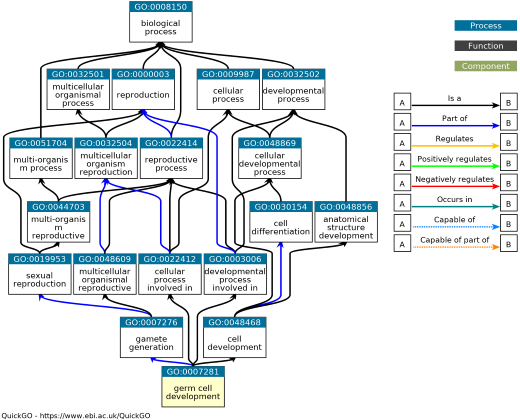
\includegraphics{go-dag}
    \caption{生殖细胞发育对应的GO示意图}
    \label{fig:go-dag}
\end{figure}

通常情况下,蛋白质复合物中蛋白质倾向于相同的功能表达,同时功能表达相似性越高时,蛋白质产生相互作用的可能性越大。部分算法\cite{ulitsky_identification_2007,jianxing_feng_max-flow-based_2011}基于功能表达数据提出了$PIN$连边权重更新的方法。
本文采用两种方法计算蛋白质功能相似度,将计算结果作为$PIN$网络中邻边的蛋白质功能特征。

第一种蛋白质功能相似度计算方法为Wang等人\cite{wang_new_2007}提出的方法。

给定一个GO注释项$p$,从GO的总体DAG图中提取子图$DAG_p(A,T_p,E_p)$,其中$T_p$是$p$及所有$p$的祖先结点的注释项,$E_p$表示所有截取的注释项的连接关系。
定义$T_p$中每一个结点对$p$的语义值如下:
\begin{equation}
    \label{equ:feat:go:SAT}
    S_p(t)=\left\{\begin{array}{l}
        1,t=p                                                                        \\
        \max {\{ w_e\times S_p(t^\prime )| t^\prime\in ~children~of~(t) \} },t\neq p \\
    \end{array}\right.
\end{equation}
其中$w_e$是$t^\prime$和$t$之间的权重,定义两种类型的边$is\_a$和$part\_of$权重各自为0.8和0.6。有公式可以直观得出,祖先结点点中离$p$注释越远的注释项,其对$p$的语义值越小,而$p$对自身的语义值贡献为1。
定义了所有祖先结点对$p$的语义值之后,可以直接得出$p$的语义值得分,计算公式如下:
\begin{equation}
    \label{equ:feat:go:SVA}
    SV(p)=\sum_{t \in T_p}(t)
\end{equation}
按照该计算方法,可以得到每一个注释项各自的语义值,在此基础上可以得到两个注释项$p$,$q$语义值的相似度,具体计算方法如下:
\begin{equation}
    \label{equ:feat:go:SimItemWang}
    Sim_{GO}(p,q)=\frac{\sum_{t \in T_p \cap T_q}(S_p(t)+S_q(t))}{SV(p)+SV(q)}
\end{equation}
其中$t$为$p$和$q$的所有公共祖先结点。由于蛋白质通常是由多个注释项组成,因此蛋白质之间的功能相似性需要考虑两个蛋白质各自注释项之间的综合结果,其具体计算方法如下:
\begin{equation}
    \label{equ:feat:go:SimProteinWang}
    \begin{aligned}
        Sim_{Protein}(P,Q) & =\frac{1}{m+n}\cdot \left\{\sum_{1\leq i\leq m}{\max_{1\leq j\leq n}[{Sim_{GO}(p_i,q_j)}}]\right. \\
                           & \left.+\sum_{1\leq j\leq n}{\max_{1\leq i\leq m}[{Sim_{GO}(p_i,q_j)}}]\right\}
    \end{aligned}
\end{equation}
其中$P$,$Q$表示两个蛋白质,其中分别具有$\{p_i| i=1,2,\dots,m\}$,$\{q_j| j=1,2,\dots,n\}$的功能注释项。
这个方法的核心思想是将两个蛋白质的注释信息相互关系矩阵$m\times n$构造出来,只考虑源蛋白质的某一个注释项和目标蛋白质所有注释项最大的相关性,而蛋白质的相互作用关系是所有最大值的平均。

第二种蛋白质功能相似度计算方法为Lin等人\cite{lin_information-theoretic_1998}提出的方法。首先计算某两个注释项之间的相关性,具体计算过程如下:
\begin{equation}
    \label{equ:feat:go:SimItemLin}
    Sim_{GO}(p,q)=\min_{anc \in Ancient(p,q)}\mathcal{P} (anc)
    % Sim_{GO}(p,q)=\max{\frac{2\times \log }{} }
\end{equation}
其中$Ancient(p,q)$表示两个注释项的公共祖先,而$\mathcal{P}$表示某一个注释项在所有蛋白质中出现的概率。这个计算公式直观的认为,两个具有相互关联的功能注释,其关联结点越稀有,则表示两个注释项的相关性越强。计算蛋白质功能相似性的计算方法如下:
\begin{equation}
    \label{equ:feat:go:SimProteinLin}
    Sim_{Protein}(P,Q)=\max{\frac{2\times \log \{Sim_{GO}(p,q)\}}{\log {\mathcal{P}_p}+\log {\mathcal{P}_q}} }
\end{equation}


\subsection{蛋白质结构域特征}
\label{subsection:domainSimilarity}
蛋白质结构域时蛋白质具有独立功能和特异结构的区域,结构域互作信息影响蛋白质复合物的形成\cite{kim_relating_2006}。结构域之间具有相互作用关系,这些相互作用关系可以从三维交互域(3did)数据库\cite{mosca_3did_2014}提取,并构建成结构域相互作用网络(Domain-Domain Interaction Network,简称DDI)。
单个蛋白质所具有的结构域可以映射到结构域互作网络的若干结点,成为一个结构域集群,而蛋白质域相似性可以转换为两个结构域集群的相互作用关系。
本文中两个蛋白质的结构域互作特征包括如下方面:两个蛋白质结构域交集、并集以及相互之间的差集;映射到结构域相互网络之后,两个结构域集群之间的相互作用关系数量,其具体的计算公式如下。
\begin{equation}
    \label{equ:feat:domain}
    Sim_{domain} = \sum_{i \in dom(p)}{\sum_{j \in dom(q)}{Weight_{ij}}}
\end{equation}
其中$i$、$j$分别时蛋白质$p$、$q$之间的结构域,$Weight_{ij}$代表结构域$i$、$j$在结构域相互作用网络中的作用强度,对于无权网络可以取值为1。

huang等人\cite{huang_protein-protein_2013}在运用结构域相互作用网络预测蛋白质相互作用时,提出了使用一阶邻居和二阶邻居计算$domain$相似性的想法,其扩展方式如图\ref{fig:domain-second}所示。本文也同时补充了一阶和二阶扩展之后的蛋白质$domain$相似性特征。
\begin{figure}[htbp]
    \centering
    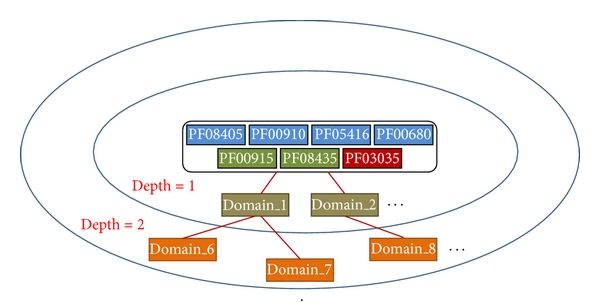
\includegraphics{domain-second}
    \caption{DDI多阶邻居示意图}
    \label{fig:domain-second}
\end{figure}


\subsection{蛋白质亚细胞特征}
\label{subsection:SubcellSimilarity}
细胞是一个高度有序的结构,胞内根据空间分布和功能不同,可以分成不同细胞器或细胞区域,蛋白质只有转运到正确的部位才能参与细胞的各种生命活动,ZHANG等人\cite{zhang_protein_2007}认为蛋白质的亚细胞定位有助于研究蛋白质的生物学功能,同时对蛋白质的其他研究如相互作用、进化等也能提供必要的信息。huang等人提出\cite{huang_genome-wide_2017}使用蛋白质复合物和亚细胞定位信息预测关键蛋白质,蛋白质复合物,蛋白质复合物的生成和功能实现和其所处的细胞位置相关,因此蛋白质的亚细胞定位能对蛋白质复合物的形成产生一定的影响。本文将两个蛋白质亚细胞定位数据的交集和并集作为蛋白质的亚细胞定位特征。图\ref{fig:subcell}为苏氨酸蛋白激酶TOR1亚细胞定位图,其中黄色的部分表示其主要的注释区域,包括细胞膜和液膜。

\begin{figure}[htbp]
    \centering
    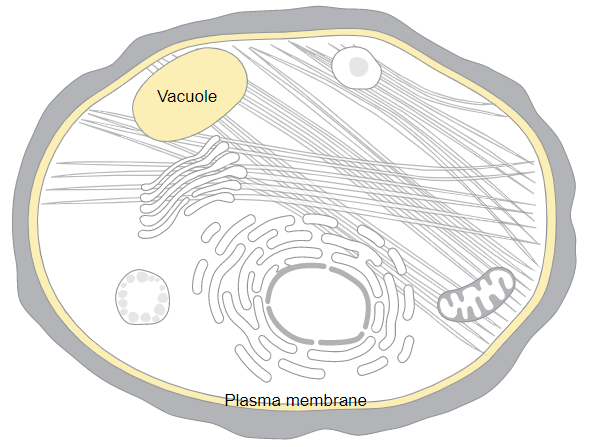
\includegraphics{subcell}
    \caption{苏氨酸蛋白激酶TOR1亚细胞定位图}
    \label{fig:subcell}
\end{figure}

\subsection{蛋白质拓扑特征}
\label{subsection:TopoSimilarity}


\section{PIN及数据集构建}
\label{section:datasetsConstruct}
\subsection{网络结构构建}
\label{subsection:NetConstruc}
\subsection{数据集提取与划分}
\label{subsection:datasetExtract}
\subsection{子图特征}
\label{subsection:subgraphFeat}

\section{相关评价指标}
\label{section:metrix}